\section{Type Switching}
\label{sec:copc}

%While \Cpp{} does not have direct support for algebraic data types, they can be 
%encoded with classes in a number of ways. One common such encoding is to 
%introduce an abstract base class representing an algebraic data type with 
%several derived classes representing variants. The variants can be 
%discriminated with either run-time type information (\emph{polymorphic 
%encoding}) or a unique tag inside a dedicated member of the common base class 
%(\emph{tagged encoding}).

\emph{Mach7} explicitly supports at least two encodings of algebraic
datatypes: runtime type information discriminant, and numerical tag
data member shared by all classes in a given hierarchy.  The library
handles them differently to let 
the user choose between openness and efficiency. The type switch for tagged 
encoding (\textsection\ref{sec:cotc}) is simpler and more efficient for many typical use cases, however, 
making it open eradicates its performance advantages (\textsection\ref{sec:cmp}). 
%The difference in 
%performance is the price we pay for keeping the solution open. We describe pros 
%and cons of each approach in \textsection\ref{sec:cmp}.

%The core of the proposal relies on two key aspects of \Cpp{} implementations:
%\begin{enumerate}
%\item a constant-time access to the virtual table pointer embedded in an object of
%  dynamic class type;
%\item injectivity of the relation between an object's inheritance path
%  and the virtual table pointer extracted from that object.
%\end{enumerate}

%\subsection{An Attractive Non-Solution}
\label{sec:cotc}

%The memoization device outlined in \textsection\ref{sec:memdev} can, in principle, also be 
%applied to tagged classes. The dynamic cast will be replaced by a small 
%compile-time template meta-program that checks whether the class associated with 
%the given tag is derived from the target type of the case clause. If so, a static 
%cast can be used to obtain the offset.

%Despite its straightforwardness, we felt that it should be possible to do better 
%than the general solution, given that each class is already identified with a 
%dedicated constant known at compile time.

While Wirth' linked list encoding was considered slow for subtype testing, it can 
be adopted for quite efficient type switching on a class hierarchy with no 
repeated inheritance. The idea is to combine fast switching on closed 
algebraic datatypes with a loop that tries the tags of base classes when 
switching on derived tags fails.

%The nominal subtyping of \Cpp{} effectively gives every class multiple types. The 
%idea is thus to associate with the type not only its most-derived tag, but also 
%the list of tags of all its base classes. In a compiler implementation such a 
%list can be stored inside the virtual table of a class, while in our library 
%solution it is shared between all the instances with the same most-derived tag 
%in a less efficient global map, associating the tag to its tag list.

For simplicity of presentation we assume a pointer to an array of tags be available 
directly through the subject's \code{taglist} data member. The array is of 
variable size: its first element is always the tag of the subject's dynamic 
type, while its end is marked with a dedicated \code{end_of_list} marker, 
distinct from all the tags. The tags in between are topologically sorted 
according to the subtyping relation with incomparable siblings listed in 
\emph{local precedence order} -- the order of the direct base classes used in 
the class definition. The list resembles the \emph{class precedence list} of 
object-oriented descendants of Lisp (e.g. Dylan, Flavors, LOOPS, and CLOS) used 
there for \emph{linearization} of class hierarchies. 
We also assume the tag-constant associated with a class \code{Di} is accessible 
through a static member \code{Di::class_tag}. These simplifications are not 
essential and the library does not rely on any of them.
%Instead, the user can retroactively narrate to the library the specific tag 
%encoding used through a trait-like class.

A type switch, below, %, built on top of a hierarchy of tagged classes, 
proceeds as 
a regular switch on the subject's tag. If the jump succeeds, we found an exact 
match; otherwise, we get into a default clause that obtains the next tag in the
list and jumps back %to the beginning of the switch statement 
for a rematch:

\begin{lstlisting}[keepspaces]
    size_t attempt = 0; 
    size_t tag = subject->taglist[attempt];
ReMatch:
    switch (tag) {
    default:
        tag = subject->taglist[++attempt];
        goto ReMatch;
    case end_of_list: 
        break;
    case D1::class_tag: 
        D1& match = static_cast<D1&>(*subject); s1;
        break;
        ...
    case Dn::class_tag: 
        Dn& match = static_cast<Dn&>(*subject); sn;
        break;
    }
\end{lstlisting}

\noindent
The above structure, which we call a \emph{tag switch}, implements a variation of 
best-fit semantics based on local precedence order. It lets us dispatch to the case 
clause of the most-specialized class with an overhead of initializing two 
local variables, compared to an efficient switch used on algebraic data types. 
Dispatching to a case clause of a base class will take time roughly proportional 
to the distance between the matched base class and the derived class in the 
inheritance graph, thus the technique is not constant. When none of the base 
class tags was matched, we will necessarily reach the end\_of\_list marker %in the list 
and exit the loop. %As mentioned before, 
The default clause, %of the type switch 
again, can be implemented with a case clause on the subject type's tag: \code{case S::class_tag:}

The efficiency of the above code crucially depends on the set of tags 
being small and sequential to justify the use of a jump table instead of a
decision tree to implement the switch. This is usually not a problem in closed 
hierarchies based on tag encoding since the designer of the hierarchy handpicks 
the tags herself. The use of a static cast %to obtain proper reference once the most specialized derived class has been established, 
however, essentially limits the use of 
this mechanism to non-repeated inheritance only. This only refers to the way target 
classes inherit from the subject type -- they can freely inherit from other classes. 
%as long as they inherit the subject type through non-repeated inheritance only. 
Due to these restrictions, the technique is not open because it may  
violate independent extensibility. We discuss in \textsection\ref{sec:cmp} that 
making the technique more open will also eradicate its performance advantages.


\subsection{An Open but Inefficient Solution}
\label{sec:poets}

Instead of starting with an efficient solution and trying to make it open, we 
start with an open solution and try to make it efficient. The following 
cascading-if statement implements the first-fit semantics for our type switch in 
a truly open fashion:

\begin{lstlisting}
if (T1* match=dynamic_cast<T1*>(subject)) {s1;} else
if (T2* match=dynamic_cast<T2*>(subject)) {s2;} else
...
if (Tn* match=dynamic_cast<Tn*>(subject)) {sn;}
\end{lstlisting}

\noindent
Despite the obvious simplicity, its main drawback is performance: a typical implementation of 
\code{dynamic_cast} takes time proportional to the distance between base and 
derived classes in the inheritance tree. What is worse is that due to the
sequential order of tests, the time to uncover the type in the $i^{th}$ case 
clause will be proportional to $i$, while failure to match will take the longest. 
This linear increase can be seen in the Figure~\ref{fig:DCastVis1}, where 
the above cascading-if was applied to a flat hierarchy encoding an algebraic 
data type with 100 variants. The same type-switching functionality implemented 
with the visitor design pattern took only 28 cycles regardless of the 
case.\footnote{Each case $i$ was timed multiple times, thus turning the experiment 
into a repetitive benchmark described in \textsection\ref{sec:eval}. In a more
realistic setting, represented by random and sequential benchmarks, the cost of 
double dispatch was varying between 52 and 55 cycles.}
This is more than 3 times faster than the 93 cycles it took to uncover even the 
first case with \code{dynamic_cast}, while it took 22760 cycles to uncover the 
last.
In a test involving a flat hierarchy of 100 variants, it took 93 cycles to 
discover the first type and 22760 to discover the last (with their linear combination 
for the types in between). A visitor design pattern could 
uncover any type in about 55 cycles, regardless of its position among the case 
clauses, while a switch based on sequential tags could achieve the same in less 
than 20 cycles. The idea is thus to combine the openness of the above structure 
with the efficiency of a jump table on small sequential values.

Relying on \code{dynamic_cast} also makes an implicit semantic choice where we 
are no longer looking for the first/best-fitting type that is in subtyping 
relation, but for the first/best-fitting type to which a cast is possible from 
the source subobject (\textsection\ref{sec:specifics}).

\begin{figure}[htbp]
  \centering
    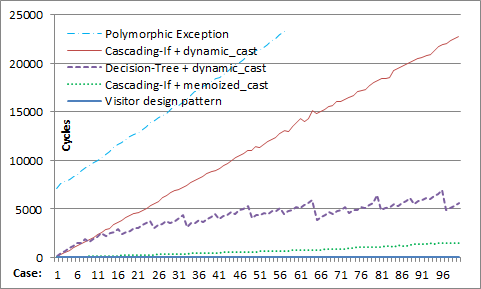
\includegraphics[width=0.47\textwidth]{DCast-vs-Visitors1.png}
  \caption{Type switching based on na\"ive techniques}
  \label{fig:DCastVis1}
\end{figure}

%Seeing several solutions whose time increases with the position of the case 
%clause in the type switch, one may wonder how many such clauses a typical 
%program might have. A program dealing with abstract syntax trees in 
%Pivot~\cite{Pivot09} that we implemented using our pattern-matching library had 
%8 match statements with 5, 7, 8, 10, 15, 17, 30 and 63 case clauses, 
%respectively. With Pivot having the smallest number of node kinds among the 
%compiler frameworks we had a chance to work with, we expect a similar or larger 
%number of case clauses in other compiler applications.

When the class hierarchy is not flat and has several levels, the above cascading-if can be replaced 
with a decision tree that tests base classes first and thus eliminates many of 
the derived classes from consideration. This approach is used by Emir to deal with 
type patterns in Scala~\cite[\textsection 4.2]{EmirThesis}. The intent is to 
replace a sequence of independent dynamic casts between classes that are far 
from each other in the hierarchy with nested dynamic casts between classes that 
are close to each other. Another advantage is the possibility to fail early: 
if the type of the subject does not match any of the clauses, we will not have to try all the cases. 
A flat hierarchy, which will likely be formed by the leaves in even a multi-level 
hierarchy, will not be able to benefit from this optimization and 
will effectively degrade to the above cascading-if. Nevertheless, when 
applicable, the optimization can be very useful and its benefits can be seen in
Figure~\ref{fig:DCastVis1} under ``Decision-Tree + dynamic\_cast''. The class 
hierarchy for this timing experiment formed a perfect binary tree with 
classes number 2*N and 2*N+1 derived from a class with number N. The structure 
of the hierarchy also explains the repetitive pattern of timings.

The above solution either in a form of cascading-if or as a decision tree can be 
significantly improved by lowering the cost of a single \code{dynamic_cast}. 
We devised an asymptotically constant version of this operator that we call
\code{memoized_cast} in \textsection\ref{sec:memcast}. As can be seen 
from the graph titled ``Cascading-If + memoized\_cast'', it speeds up the 
above cascading-if solution by a factor of 18 on average, as well as outperforms 
the decision-tree based solution with dynamic\_cast for a number of case clauses 
way beyond those that can happen in a reasonable program. 
We leave the discussion of the technique until 
\textsection\ref{sec:memcast}, while we keep it in the chart to give perspective on 
an even faster solution to dynamic casting. The slowest implementation in the 
chart based on exception handling facilities of C++ is discussed in 
\textsection\ref{sec:xpm}.

The approach of Gibbs and Stroustrup~\cite{FastDynCast} employs divisibility of numbers to obtain a 
tag allocation scheme capable of performing type testing in constant time. 
Extended with a mechanism for storing offsets required for this-pointer 
adjustments, the technique can be used for extremely fast dynamic casting on 
quite large class hierarchies. The idea is to allocate tags 
for each class in such a way that tag of a class D is divisible by a tag of a 
class B if and only if class D is derived from class B. For comparison purposes 
we hand crafted this technique on the above flat and binary-tree hierarchies and 
then redid the timing experiments from Figure~\ref{fig:DCastVis1} using the fast 
dynamic cast. The results are presented in Figure~\ref{fig:DCastVis2}. For 
reference purposes we retained ``Visitor Design Pattern'' and ``Cascading-If + 
memoized\_cast'' timings from Figure~\ref{fig:DCastVis1} unchanged. Note that 
the Y-axis has been scaled-up 140 times, which is why the slope of 
``Cascading-If + memoized\_cast'' timings is so much steeper.

\begin{figure}[htbp]
  \centering
    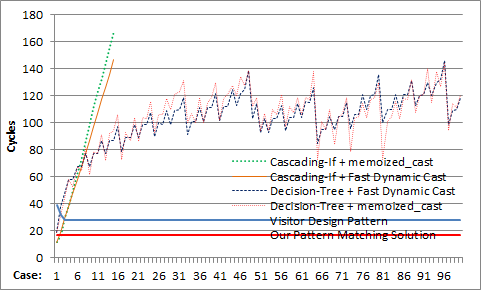
\includegraphics[width=0.47\textwidth]{DCast-vs-Visitors2.png}
  \caption{Type switching based on the fast dynamic cast of Gibbs and Stroustrup~\cite{FastDynCast}}
  \label{fig:DCastVis2}
\end{figure}

As can be seen from the figure the use of our memoized\_cast implementation can 
get close in terms of performance to the fast dynamic cast, especially 
when combined with decision trees. An important difference that cannot be seen 
from the chart, however, is that the performance of memoized\_cast is 
asymptotic, while the performance of fast dynamic cast is guaranteed. This 
happens because the implementation of memoized\_cast will incur an overhead of 
a regular dynamic\_cast call on every first call with a given most derived type. 
Once that class is memoized, the performance will remain as shown. Averaged over 
all calls with a given type we can only claim we are asymptotically as good as 
fast dynamic cast.

Unfortunately fast dynamic casting is not truly open to fully satisfy our 
checklist. The structure of tags required by the scheme limits the number of 
classes it can handle. A 32-bit integer is estimated to be able to represent 7 
levels of a class hierarchy that forms a binary tree (255 classes), 6 levels of 
a similar ternary tree hierarchy (1093 classes) or just one level of a hierarchy 
with 9 base classes -- multiple inheritance is the worst case scenario of the 
scheme that quickly drains its allocation possibilities. Besides, similarly to 
other tag allocation schemes, presence of class extensions in \emph{Dynamically Linked Libraries} (DLLs) will likely 
require an integration effort to make sure different DLLs are not reusing prime 
numbers in a way that might result in an incorrect dynamic cast.

A number of other constant-time techniques for class-membership testing is 
surveyed by Gil and Zibin~\cite[\textsection 4]{PQEncoding}. They are intended 
for type testing, and thus will have to be combined with decision trees 
for type switching, resulting in similar to fast dynamic cast performance. 
They too assume access to the entire class hierarchy at compile time and thus 
are not open.

In view of the predictably-constant dispatching overhead of the visitor design pattern, 
it is clear that any open solution that will have a non-constant dispatching 
overhead will have a poor chance of being adopted. Multi-way switch on 
sequentially allocated tags~\cite{Spuler94} was one of the few techniques that 
could achieve constant overhead, and thus compete with and even outperform visitors. 
Unfortunately the scheme has problems of its own that make it unsuitable for 
truly open type-switching and here is why.

%To better understand the problem let us look at some existing solutions to type 
%switching that we found to be used in practice. 

%From our experience on this project we have noticed that we can only compete 
%with visitors when switch statements are implemented with a jump table. As soon 
%as compiler was putting even a single branch into the decision tree of cases, 
%the performance was degraded significantly. From this perspective we do not 
%regard solutions based on decision trees as efficient, since they do not let us 
%compete compete with the visitors solution.

The simple scheme of assigning a unique tag per variant (instantiatable class 
here) will not pass our first question because the tags of base and derived 
classes will have to be different if the base class can be instantiated on its 
own. In other words we will not be able to land on a case label of a base class, while 
having a derived tag only. The already mentioned partitioning of tags of derived 
classes based on the classes in case clauses also will not help as it assumes 
knowledge of all the classes and thus fails extensibility through DLLs.

In practical implementations hand crafted for a specific class hierarchy, tags 
often are not chosen arbitrarily, but to reflect the subtyping relation of the 
underlying hierarchy. Switching on base classes in such a setting will typically 
involve a call to some function $f$ that converts derived class' tag into a base 
class' tag. An example of such a scheme would be having a certain bit in the tag 
set for all the classes derived from a given base class. Unfortunately this 
solution creates more problems than it solves.

First of all the solution will not be able to recognize an exceptional case 
where most of the derived classes should be handled as a base class, while a few 
should be handled specifically. Applying the function $f$ puts several different 
types into an equivalence class with their base type, making them 
indistinguishable from each other.

Secondly, the assumed structure of tags is likely to make the set of tags 
sparse, effectively forcing the compiler to use a decision tree instead of a jump 
table to implement the switch. Even though conditional jump is reported to be 
faster than indirect jump on many computer architectures~\cite[\textsection 
4]{garrigue-98}, this did not seem to be the case in our experiments. Splitting 
of a jump table into two with a condition, that was sometimes happening because 
of our case label allocation scheme, was resulting in a noticeable degradation of 
performance in comparison to a single jump table.

Besides, as was seen in the scheme of Gibbs and Stroustrup, the assumed 
structure of tags can also significantly decrease the number of classes a given 
allocation scheme can handle. It is also interesting to note that even though 
their scheme can be easily adopted for type switching with decision trees, it is 
not easily adoptable for type switching with jump tables: in order to obtain 
tags of base classes we will have to decompose the derived tag into primes and 
then find all the dividers of the tag present in case clauses.

Several authors had noted the relationship between exception handling and type 
switching before~\cite{Glew99,ML2000}. Not surprisingly, the exception handling 
mechanism of \Cpp{} can be abused to implement the first-fit semantics of a type 
switch statement. The idea is to harness the fact that catch-handlers in \Cpp{} 
essentially use first-fit semantics to decide which one is going to handle a 
given exception. Unfortunately the approach is even slower than the use of 
\code{dynamic_cast} and we only list it here for comparison.

To summarize, truly open and efficient type switching is a non-trivial problem. 
The approaches we found in the literature were either open or efficient, 
but not both. Efficient implementation was typically achieved by sealing the 
class hierarchy and using a jump table on sequential tags. Open implementations 
were resorting to type testing and decision trees, which was not efficient. 
We are unaware of any efficient tag allocation scheme that can be used in a 
truly open scenario.

%%%%%%%%%%%%%%%%%%%%%%%%%%%%%%%%%%%%%%5555

%\noindent
%We chose to give it a first-fit semantics in our library as it was resembling 
%pattern matching facilities of other languages and was the most intuitive. The 
%following code can be generated to implement it:
%
%\begin{lstlisting}
%if (D1* derived = dynamic_cast<D1*>(base)) { s1; } else
%if (D2* derived = dynamic_cast<D2*>(base)) { s2; } else
%...
%if (Dn* derived = dynamic_cast<Dn*>(base)) { sn; }
%\end{lstlisting}

%\noindent
%Note that leaving \code{else} out will effectively turn it into an all-fit 
%statement with enabled statements executed in lexicographical order.
%
%The above code is easy to understand but is extremely inefficient as for an 
%object of dynamic type $D_i$ we will have to perform $i-1$ dynamic casts that 
%fail first. The diagram below compares the times spent by visitors and the above 
%type switch statement to uncover the $i^{th}$ case. We postpone the discussion 
%of \code{memoized_cast} until section \textsection\ref{}, here we would only 
%like to notice that even though faster than the actual dynamic cast it also bears 
%a linear coefficient, not present in visitors.

\section{Solution for Polymorphic Classes}
\label{sec:copc}

Our handling of type switches for polymorphic and tagged encodings differs 
with each having its pros and cons described in details in \textsection\ref{sec:cmp}.
In this section we will concentrate on the truly open type switch for 
polymorphic encoding. The type switch for tagged encoding (\textsection\ref{sec:cotc}) 
is simpler and more efficient, however, making it open will eradicate its 
performance advantages. The difference in performance is the price we pay for 
keeping the solution open.  The core of the proposal relies on two key
aspects of C++ implementations:
\begin{enumerate}
\item a constant-time access to the virtual table pointer embedded in an object of
  dynamic class type;
\item injectivity of the relation between an object's inheritance path
  and the virtual table pointer extracted from that object.
\end{enumerate}

\subsection{A Memoization Device}
\label{sec:memdev}

Let us look at a slightly more general problem than type switching. Consider a 
generalization of the switch statement that takes predicates on a subject as its 
clauses and executes the first statement $s_i$ whose predicate is enabled: 

\begin{lstlisting}[keepspaces]
switch (x)
{
    case P1(x): s1;
    ...
    case Pn(x): sn;
}
\end{lstlisting}

\noindent
Assuming that predicates are \emph{functional} (i.e. do not involve any side 
effects), the next time we execute the switch with the same value $x$, the same 
predicate will be enabled first. We thus would like to avoid evaluating 
preceding predicates and jump to the statement it guards. In a way, we 
would like the switch to memoize the case enabled for a given $x$. 

The idea is to generate a simple cascading-if statement interleaved with jump 
targets and instructions that associate the original value with enabled target. 
The code before the statement looks up whether the association for a given value 
has already been established, and, if so, jumps directly to the target; otherwise, 
the sequential execution of the cascading-if is started. To ensure 
that the actual code associated with the predicates remains unaware of this 
optimization, the code preceding it after the target must re-establish any 
invariant guaranteed by sequential execution (\textsection\ref{sec:vtblmem}).

Described code can be easily produced in a compiler setting, but generating it in 
a library is a challenge. Inspired by Duff's Device~\cite{Duff}, 
we devised a construct that we call \emph{Memoization Device} doing just 
that in standard \Cpp{}:

\begin{lstlisting}
typedef decltype(x) T; // T is the type of subject x
static std::unordered_map<T,size_t> jump_targets;

switch (size_t& jump_to = jump_targets[x]) {
default: // entered when we have not seen x yet
    if (P1(x)) { jump_to = 1; case 1: s1; } else 
    if (P2(x)) { jump_to = 2; case 2: s2; } else
 ...
    if (Pn(x)) { jump_to = @$n$@; case @$n$@: sn; } else
                jump_to = @$n+1$@;
case @$n+1$@: // none of the predicates is true on x
}
\end{lstlisting}

\noindent
The static \code{jump_targets} hash table will be allocated upon first entry 
to the function. The map is initially empty and according to its logic, 
request for a key $x$ not yet in the map will allocate a 
new entry with its associated data default initialized (to 0 for \code{size_t}). Since 
there is no case label 0 in the switch, the default case will be taken, which, in 
turn, will initiate sequential execution of the interleaved cascading-if 
statement. Assignments to \code{jump_to} effectively establish association 
between value $x$ and corresponding predicate, since \code{jump_to} is a 
reference to \code{jump_targets[x]}. The last assignment records absence of 
enabled predicates for $x$.

The sequential execution of the cascading-if statement will keep checking 
predicates $P_j(x)$ until the first predicate $P_i(x)$ that returns true. By 
assigning $i$ to \code{target} we will effectively associate $i$ with $x$ since 
\code{target} is just a reference to \code{jump_target_map[x]}. This association 
will make sure that the next time we are called with the value $x$ we will jump 
directly to the label $i$. When none of the predicates returns true, we will 
record it by associating $x$ with $N+1$, so that the next time we can jump 
directly to the end of the switch on $x$. 

The above construct effectively gives the entire statement first-fit semantics. 
In order to evaluate all the statements whose predicates are true, and thus 
give the construct all-fit semantics, we might want to be able to preserve the 
fall-through behavior of the switch. In this case we can still skip the initial 
predicates returning false and start from the first successful one. This can be 
easily achieved by removing all else statements and making if-statements 
independent as well as wrapping all assignments to \code{target} with a condition, 
to make sure only the first successful predicate executes it:

\begin{lstlisting}
if (Pi(x)) { if (jump_to == 0) jump_to = @$i$@; case @$i$@: si; }
\end{lstlisting}

\noindent
Note that the protocol that has to be maintained by this structure does not 
depend on the actual values of case labels. We only require them to be 
different and include a predefined default value. The default clause can be 
replaced with a case clause for the predefined value, but keeping the default  
clause generates faster code. A more important consideration is to 
keep the values close to each other. Not following this rule might result in a 
compiler choosing a decision tree over a jump table implementation of the 
switch, which in our experience significantly degrades the performance.

The first-fit semantics is not an inherent property of the memoization device. 
Assuming that the conditions are either mutually exclusive or imply one another, we 
can build a decision-tree-based memoization device that will effectively have 
\emph{most-specific} semantics -- an analog of best-fit semantics in predicate 
dispatching~\cite{ErnstKC98}.

Imagine that the predicates with the numbers $2i$ and $2i+1$ are mutually exclusive and 
each imply the value of the predicate with number $i$, i.e.
$\forall i\forall x\in\bigcap_j\mathsf{Domain}(P_j).P_{2i+1}(x)\rightarrow P_i(x)\wedge P_{2i}(x)\rightarrow P_i(x)\wedge\neg(P_{2i+1}(x)\wedge P_{2i}(x))$ holds. 
Examples of such predicates are class membership tests where the truth of 
testing membership in a derived class implies the truth of testing membership in 
its base class.

The following decision-tree-based memoization device will execute the statement 
$s_i$ associated with the \emph{most-specific} predicate $P_i$ (i.e. the 
predicate that implies all other predicates true on $x$) that evaluates to true 
or will skip the entire statement if none of the predicates is true on $x$.

\begin{lstlisting}
switch (size_t& jump_to = jump_targets[x]) {
default:
    if (P1(x)) {
        if (P2(x)) {
            if (P4(x)) { jump_to = 4; case 4: s4; } else
            if (P5(x)) { jump_to = 5; case 5: s5; } 
            jump_to = 2; case 2: s2;
        } else
        if (P3(x)) {
            if (P6(x)) { jump_to = 6; case 6: s6; } else
            if (P7(x)) { jump_to = 7; case 7: s7; } 
            jump_to = 3; case 3: s3;
        }
        jump_to = 1; case 1: s1;
    } else { jump_to = 0; case 0: ; }
}
\end{lstlisting}

\noindent
An example of predicates that satisfy this condition are class membership tests
where the truth of a predicate that tests membership in a derived class implies 
the truth of a predicate that tests membership in its base class. 
Our library solution prefers the simpler cascading-if approach only because the 
necessary code structure can be laid out with macros. A compiler solution 
will use the decision-tree approach whenever possible to lower the cost of the 
first match from linear in case's number to logarithmic as seen in Figure\ref{fig:DCastVis1}.

When the predicates do not satisfy the implication or mutual exclusion properties 
mentioned above, a compiler of a language based on predicate dispatching would 
typically issue an ambiguity error. Some languages might choose to resolve it 
according to lexical or some other ordering. In any case, the presence of 
ambiguities or their resolution has nothing to do with memoization device 
itself. The latter only helps optimize the execution once a particular choice of 
semantics has been made and code implementing it has been laid out.

The main advantage of the memoization device is that it can be built around 
almost any code, providing that we can re-establish the invariants guaranteed 
by sequential execution. Its main disadvantage is the size of the hash table 
that grows proportionally to the number of different values seen. Fortunately, 
the values can often be grouped into equivalence classes that do not change the 
outcome of the predicates. The map can then associate the equivalence class of a 
value with a target instead of associating the value with it. 

In application to type switching, the idea is to use the memoization device to 
learn the outcomes of type inclusion tests (with \code{dynamic_cast} used as a 
predicate). The objects can be grouped into equivalence classes based on their 
dynamic type: the outcome of each type inclusion test will be the same on 
all the objects of the same dynamic type. We can use the  
address of a class' \code{type_info} object obtained in constant time with the
\code{typeid()} operator as a unique identifier of each dynamic type. 
Presence of multiple \code{type_info} objects for the same class, as is often 
the case when dynamic linking is involved, is not a problem, as it would 
effectively split a single equivalence class into multiple ones. 

This could have been a solution if we were only interested in class membership. 
More often than not, however, we will be interested in obtaining a reference to 
the target type of the subject, and we saw in \textsection\ref{sec:specifics} 
that the cast between the source and target subobjects depends on 
the position of the source subobject in the dynamic type's subobject graph. 
We thus would like to have different equivalence classes for different 
subobjects, but there seems to be no easy way of identifying them given just an object descriptor.

\subsection{Virtual Table Pointers}
\label{sec:vtp}

%In this section we show that under certain conditions the compiler cannot share 
%the same virtual tables between different classes or their subobjects. This 
%allows us to use virtual table pointers to \emph{uniquely} identify the 
%subobjects within the most-derived class.

Before we discuss our solution we would like to talk about certain properties of 
the C++ run-time system that we rely on. In particular,
we show that under certain conditions the compiler cannot share 
the same virtual tables between different classes or subobjects of the same 
class. This allows us to use virtual table pointers to \emph{uniquely} identify 
the subobjects within the most derived class.

Strictly speaking, the C++ standard~\cite{C++0x} does not require implementations 
to use any specific technique (e.g. virtual tables) to implement virtual functions, 
however interoperability requirements have forced many compiler vendors to design a 
set of rules called Common Vendor Application Binary Interface (the C++ 
ABI)~\cite{C++ABI}. Most C++ compilers today follow these rules, with the 
notable exception of Microsoft Visual C++. The technique presented here will 
work with any C++ compiler that follows the C++ ABI. Microsoft's own ABI is not 
publically available and thus we cannot formally verify that it satisfies 
our requirements. Nevertheless, we did run numerous experiments with various 
class hierarchies and have sufficient confidence that our approach can be used 
in Visual C++. This is why we include experimental results for this compiler as 
well.

Besides single inheritance, which is supported by most object-oriented languages, 
C++ supports multiple-inheritance of two kinds: repeated and virtual (shared). 
\emph{Repeated inheritance} creates multiple independent subobjects of the same 
type within the most derived type. \emph{Virtual inheritance} creates only one 
shared subobject, regardless of the inheritance paths. Because of this 
peculiarity of the C++ type system it is not sufficient to talk only about the 
static and dynamic types of an object -- one has to talk about a 
\emph{subobject} of a certain static type accessible through a given inheritance 
path within a dynamic type.

\begin{figure}[tbp]
  \centering
    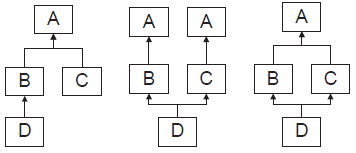
\includegraphics[width=0.47\textwidth]{Hierarchies.png}
  \caption{Single inheritance, repeated multiple inheritance and virtual multiple inheritance}
  \label{fig:hierarchy}
\end{figure}

\noindent
Note that the above picture portrais subobject relatedion, not the inheritance.

Figure~\ref{fig:objlayout} shows a typical object layout generated by a \Cpp{} 
compiler for class \code{D} from Figure~\ref{fig:inheritance}(1) under repeated 
(1) and virtual (2) inheritance of \code{A}. The layouts represent an encoding 
of the corresponding subobject graphs from Figures \ref{fig:inheritance}(2a) and 
\ref{fig:inheritance}(2b) respectively.

\begin{figure}[htbp]
  \centering
    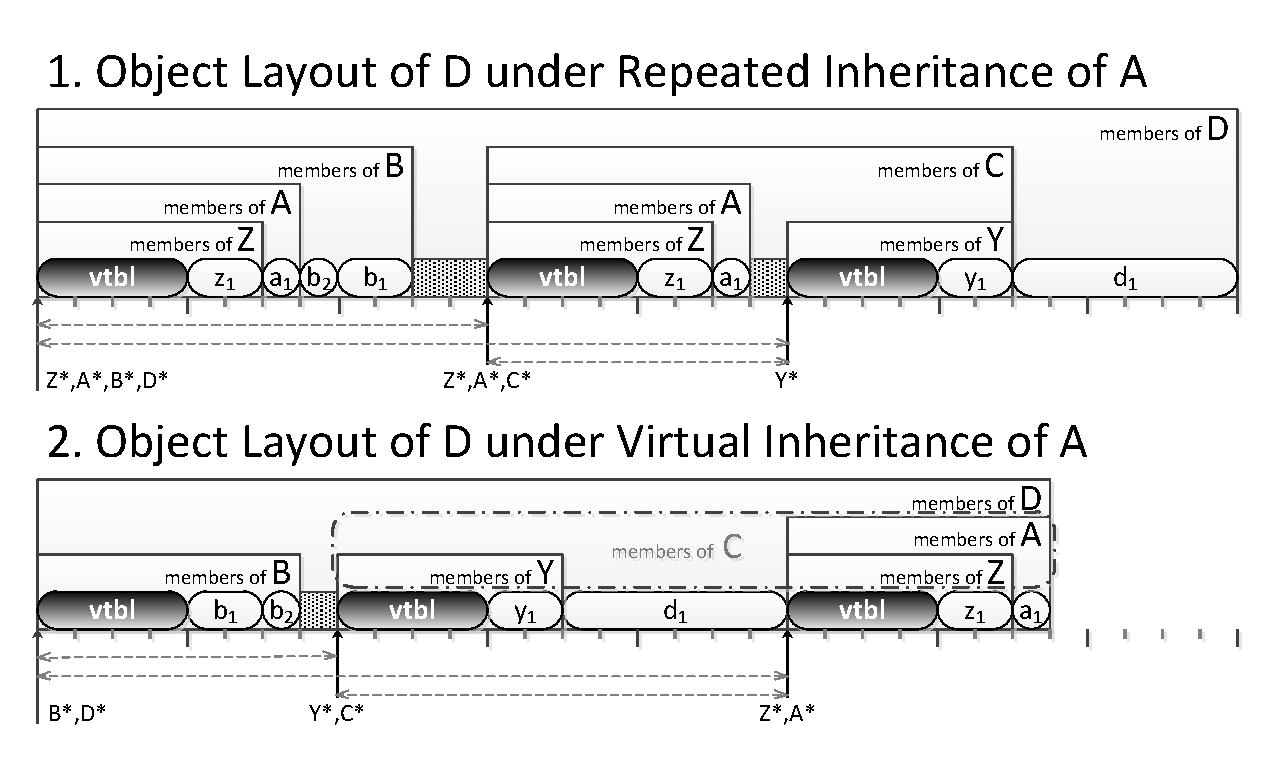
\includegraphics[width=0.47\textwidth]{obj-layout.pdf}
  \caption{Object Layout under Multiple Inheritance}
  \label{fig:objlayout}
\end{figure}

Due to the extensibility of classes, the layout decisions for classes must be 
made independently of their derived classes -- a property of the \Cpp{} object 
model that we will refer to as \emph{layout independence}. In turn, the layout of derived   
classes must conform to the layout of their base classes relatively to the offset 
of the base class within the derived one. For example, the layout of \code{A} in 
\code{C} is exactly the same as the layout of \code{A} in \code{B} and is simply
the layout of \code{A}. Base classes inherited virtually do not contribute to 
the fixed layout because they are looked up indirectly at run-time; however, 
they are not exempt from layout independence, since their lookup rules are 
agnostic of the concrete dynamic type.
%Because of this indirection, the use of virtual inheritance incures slight 
%overhead at run-time. 

Under non-virtual inheritance, members of the base class are typically laid out 
before the members of derived class, resulting in the base class being at the 
same offset as the derived class itself. In our example, the offset of \code{A} 
in \code{B} under regular (non-virtual) inheritance of \code{A} is 0.
Under multiple inheritance, different base classes might be at different offsets 
in the derived class, which is why pointers of a given static type may be 
pointing only to certain subobjects in it. These positions are marked in the 
picture with vertical arrows decorated with the set of pointer types whose 
values may point into that position. Run-time conversions between such pointers 
represent casts between subobjects of the same dynamic type and may require 
adjustments to this-pointer (shown with dashed arrows) for type safety.

A class that declares or inherits a virtual function is called a 
\emph{polymorphic class}. The \Cpp{} standard~\cite{C++11} does not prescribe any 
specific implementation technique for virtual function dispatch.
However, in practice, all \Cpp{} compilers use a strategy based on so-called
virtual function tables (or vtables for short) for efficient dispatch. 
The vtable is part of the reification of a polymorphic class type.  
\Cpp{} compilers embed a pointer to a vtable (vtbl-pointer for short) in every object of
polymorphic class type (and thus every subobject of that type inside other 
classes due to layout independence). CFront, the first \Cpp{} compiler, puts the 
vtbl-pointer 
at the end of an object. The so-called ``common vendor \Cpp{} ABI''~\cite{C++ABI} requires the 
vtbl-pointer to be at offset 0 of an object. ~\footnote{The following compilers 
are known to comply with the \Cpp{} ABI: GCC (3.x and up); Clang and llvm-g++; 
Linux versions of Intel and HP compilers, and compilers from ARM. See 
http://morpher.com/documentation/articles/abi/ for details.}. 
We do not have 
access to the unpublished Microsoft ABI, but we have experimental evidence that 
their \Cpp{} compiler also puts the vtbl-pointer at the start of an object.

While the exact offset of the vtbl-pointer within the (sub)object is not important 
for this discussion, because of layout independence every (sub)object of a 
polymorphic type \code{S} will have a vtbl-pointer at a predefined offset. 
Such offset may be different for different static types \code{S}, in which case 
the compiler will know at which offset in type \code{S} the vtbl-pointer is 
located, but it will be the same within any subobject of a static type 
\code{S}. For a library implementation we assume the presence of a function 
\code{template <typename S> intptr_t vtbl(const S* s);} 
that returns the address of the virtual table corresponding to the subobject 
pointed to by \code{s}. Such a function can be trivially implemented for the 
common vendor \Cpp{} ABI, where the vtbl-pointer is always at offset 0:

\begin{lstlisting}
template <typename S> std::intptr_t vtbl(const S* s) {
    static_assert(std::is_polymorphic<S>::value, "error");
    return *reinterpret_cast<const std::intptr_t*>(s);
}
\end{lstlisting}

\noindent
Each of the \code{vtbl} fields shown in Figure~\ref{fig:objlayout} holds a 
vtbl-pointer referencing a group of virtual methods known in the object's static 
type. Figure~\ref{fig:vtbl}(1) shows a typical layout of virtual function tables 
together with objects it points to for classes \code{B} and \code{D}.

\noindent
\begin{figure}[htbp]
  \centering
    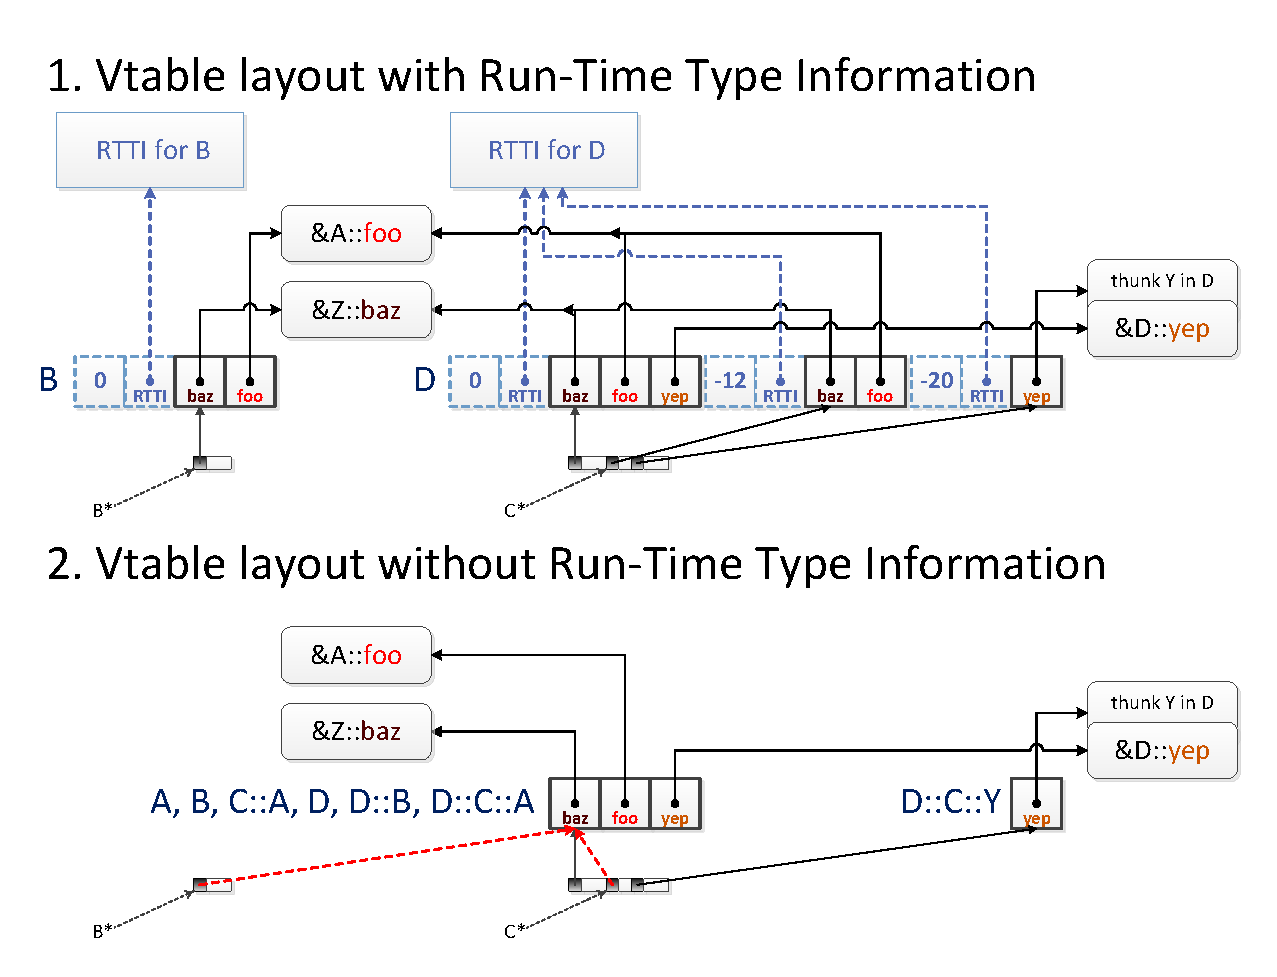
\includegraphics[width=0.49\textwidth]{v-table.pdf}
  \caption{VTable layout with and without RTTI}
  \label{fig:vtbl}
\end{figure}

Entries in the vtable to the right of the address pointed to by a vtbl-pointer 
represent pointers to functions, while entries to the left of it represent 
various additional fields like a pointer to a class' type information, offset to 
top, offsets to virtual base classes, etc. In many implementations, this-pointer 
adjustments required to dispatch properly the call were stored in the vtable 
along with function pointers. Today most implementations prefer to use 
\emph{thunks} or \emph{trampolines} -- additional entry points to a function, 
that adjust this-pointer before transferring the control to the function, -- 
which was shown to be more efficient~\cite{Driesen96}. Thunks in general may 
only be needed when virtual function is overridden. In such cases, the 
overridden function may be called via a pointer to a base class or a pointer to 
a derived class, which may not be at the same offset in the actual object.

The intuition behind our proposal is to use the values of vtbl-pointers stored 
inside the object to uniquely identify the subobject in it. There are several 
problems with the approach, however. First, the same vtbl-pointer is 
usually shared by multiple subobjects when one of them contains the other. For 
example, the first vtbl-pointer in Figure~\ref{fig:objlayout}(1) will be shared 
by objects of static type \code{Z*}, \code{A*}, \code{B*} and \code{D*}. This is 
not a problem for our purpose, because the subobjects of these types will be at 
the same offset in the object. Secondly, and more importantly, 
however, there are legitimate optimizations that let the compiler share the same 
vtable among multiple subobjects of often-unrelated types.

Generation of the \emph{Run-Time Type Information} (or RTTI for short) can 
typically be disabled with a compiler switch and the Figure~\ref{fig:vtbl}(2) 
shows the same vtable layouts once RTTI has been disabled. Since neither 
\code{baz} nor \code{foo} were overridden, the prefix of the vtable for the 
\code{C} subobject in \code{D} is exactly the same as the vtable for its 
\code{B} subobject, the \code{A} subobject of \code{C}, or the entire vtable of 
\code{A} and \code{B} classes. Such a layout, for example, is produced by 
Microsoft Visual \Cpp{} 11 when the command-line option \code{/GR-} is specified. 
The Visual \Cpp{} compiler has been known to unify code identical on binary level, 
which in some cases may result in sharing of the same vtable between unrelated 
classes (e.g. when virtual functions are empty).

%\Cpp{} supports multiple-inheritance of two kinds: repeated and virtual (shared). 
%\emph{Repeated inheritance} creates multiple independent subobjects of the same 
%type within the dynamic type. \emph{Virtual inheritance} creates only one 
%shared subobject, regardless of the inheritance paths. Consequently,
%it is not sufficient to talk only about the 
%static and dynamic types of an object -- one has to talk about a 
%\emph{subobject} of a certain static type accessible through a given inheritance 
%path within a dynamic type. 

We now would like to show more formally that in the presence of RTTI, a common vendor \Cpp{} ABI 
compliant implementation would always have all the vtbl-pointers different. To do 
so, we need a closer look at the notion of subobject, which has been formalized 
before~\cite{RF95,WNST06,RDL11}. We follow here the presentation of Ramamanandro 
et al~\cite{RDL11}.

\subsection{Subobjects}
\label{sec:subobj}

We assume a program $\mathfrak{P}$ is represented by its class table, which can be 
queried for inheritance relations between classes. All subsequent definitions 
are implicitly parameterized over a given program $\mathfrak{P}$. 
A class $B$ is a \emph{direct repeated base class} of  
$D$ if $B$ is mentioned in the list of base classes of $D$ without the 
\code{virtual} keyword ($D \prec_R B$). Similarly, a class $B$ is a \emph{direct 
shared base class} of $D$ if $B$ is mentioned in the list of base classes of $D$ 
with the \code{virtual} keyword ($D \prec_S B$). A reflexive transitive closure 
of these relationships $\preceq^*=(\prec_R \cup \prec_S)^*$ defines the 
\emph{subtyping} relation on types of program $\mathfrak{P}$.
A base class \emph{subobject} of a given \emph{complete object} is represented by a pair 
$\sigma = (h,l)$ with $h \in \{\mathsf{Repeated},\mathsf{Shared}\}$ representing the 
kind of inheritance (single inheritance is $\mathsf{Repeated}$ with one base class) and $l$ 
representing the path in a non-virtual inheritance graph.
A judgment of the form $\mathfrak{P}\vdash C\leftY\sigma\rightY A$ states that 
in a program $\mathfrak{P}$, $\sigma$ designates a subobject of static type $A$ 
within an object of type $C$. Omitting the context $\mathfrak{P}$: 

A predicate $C\leftY\sigma\rightY A$ they introduce means that $\sigma$ 
designates a subobject of static type $A$ within the most derived object of 
type $C$.

\begin{mathpar}
\inferrule
{C \prec_S B \\ B\leftY(h,l)\rightY A}
{C\leftY(\mathsf{Shared},l)\rightY A}

\inferrule
{}
{C\leftY(\mathsf{Repeated},C::\epsilon)\rightY C}

\inferrule
{C \prec_R B \\ B\leftY(\mathsf{Repeated},l)\rightY A}
{C\leftY(\mathsf{Repeated},C::l)\rightY A}
\end{mathpar}

\noindent
$\epsilon$ indicates an empty path, but we will generally omit it in writing 
when understood from the context. In the case of repeated inheritance in 
Figure~\ref{fig:inheritance}(1), an object of the dynamic class \code{D} 
will have the following $\mathsf{Repeated}$ subobjects:
\code{D::C::Y}, 
\code{D::B::A::Z}, 
\code{D::C::A::Z}, 
\code{D::B::A}, 
\code{D::C::A}, 
\code{D::B}, 
\code{D::C}, 
\code{D}.
Similarly, in case of virtual inheritance in the same example, an object of the 
dynamic class \code{D} will have the following $\mathsf{Repeated}$ subobjects:
\code{D::C::Y}, 
\code{D::B}, 
\code{D::C}, 
\code{D}
as well as the following $\mathsf{Shared}$ subobjects: 
\code{D::A::Z}, 
\code{D::Z}, 
\code{D::A}. See Figure~\ref{fig:inheritance} for illustration.

It is easy to show by structural induction on the above definition, that 
$C\leftY\sigma\rightY A \implies \sigma=(h,C::l_1) \wedge \sigma=(h,l_2::A::\epsilon)$, 
which simply means that any path to a subobject of static type $A$ within the 
object of dynamic type $C$ starts with $C$ and ends with $A$. This 
observation shows that $\sigma_\bot = (\mathsf{Shared},\epsilon)$ does not 
represent a valid subobject. If $\Sigma_\mathfrak{P}$ is the domain of all subobjects in 
the program $\mathfrak{P}$ extended with $\sigma_\bot$, then a \emph{cast} operation can be 
understood as a function $\delta : \Sigma_\mathfrak{P} \rightarrow \Sigma_\mathfrak{P}$. We use 
$\sigma_\bot$ to indicate an impossibility of a cast. The fact that $\delta$ is 
defined on subobjects as opposed to actual run-time values reflects the 
non-coercive nature of the operation, i.e. the underlying value remains the 
same. Any implementation of such a function must thus satisfy the following 
condition:
\begin{eqnarray*}
C \leftY\sigma_1\rightY A \wedge \delta(\sigma_1) = \sigma_2 \implies C \leftY\sigma_2\rightY B
\end{eqnarray*}
\noindent
i.e. the dynamic type of the value does not change during casting, only the way 
we reference it does. Following the definitions from 
\textsection\ref{sec:specifics}, $A$ is the \emph{source type} and $\sigma_1$ is 
the \emph{source subobject} of the cast, while $B$ is the \emph{target type} and 
$\sigma_2$ is the \emph{target subobject} of it. The type $C$ is the 
dynamic type of the value being casted. The \Cpp{} semantics states more 
requirements to the implementation of $\delta$: e.g. 
$\delta(\sigma_\bot) = \sigma_\bot$ etc. but their precise modeling is out of 
scope of this discussion. We would only like to point out here that since 
the result of the cast does not depend on the actual value and only on the 
source subobject and the target type, we can memoize the outcome of a cast on 
one instance in order to apply its results to another.

%Figure~\ref{fig:objlayout}(1)
%$Z\leftY(\mathsf{Repeated},      [Z])\rightY Z$,
%$A\leftY(\mathsf{Repeated},    [A,Z])\rightY Z$,
%$B\leftY(\mathsf{Repeated},  [B,A,Z])\rightY Z$,
%$D\leftY(\mathsf{Repeated},[D,B,A,Z])\rightY Z$,
%$C\leftY(\mathsf{Repeated},  [C,A,Z])\rightY Z$,
%$D\leftY(\mathsf{Repeated},[D,C,A,Z])\rightY Z$,
%$Y\leftY(\mathsf{Repeated},      [Y])\rightY Y$,  
%$C\leftY(\mathsf{Repeated},    [C,Y])\rightY Y$,
%$D\leftY(\mathsf{Repeated},  [D,C,Y])\rightY Y$,
%$A\leftY(\mathsf{Repeated},      [A])\rightY A$, 
%$B\leftY(\mathsf{Repeated},    [B,A])\rightY A$,
%$D\leftY(\mathsf{Repeated},  [D,B,A])\rightY A$,
%$C\leftY(\mathsf{Repeated},    [C,A])\rightY A$,
%$D\leftY(\mathsf{Repeated},  [D,C,A])\rightY A$,
%$B\leftY(\mathsf{Repeated},      [B])\rightY B$,
%$D\leftY(\mathsf{Repeated},    [D,B])\rightY B$,
%$C\leftY(\mathsf{Repeated},      [C])\rightY C$,
%$D\leftY(\mathsf{Repeated},    [D,C])\rightY C$,
%$D\leftY(\mathsf{Repeated},      [D])\rightY D$,
%
%Figure~\ref{fig:objlayout}(2)
%$Z\leftY(\mathsf{Repeated},      [Z])\rightY Z$,
%$A\leftY(\mathsf{Repeated},    [A,Z])\rightY Z$,
%$B\leftY(\mathsf{Shared},    [B,A,Z])\rightY Z$,
%$C\leftY(\mathsf{Shared},    [C,A,Z])\rightY Z$,
%$D\leftY(\mathsf{Shared},    [D,A,Z])\rightY Z$,
%$D\leftY(\mathsf{Shared},      [D,Z])\rightY Z$,
%$Y\leftY(\mathsf{Repeated},      [Y])\rightY Y$,  
%$C\leftY(\mathsf{Repeated},    [C,Y])\rightY Y$,
%$D\leftY(\mathsf{Repeated},  [D,C,Y])\rightY Y$,
%$A\leftY(\mathsf{Repeated},      [A])\rightY A$, 
%$B\leftY(\mathsf{Shared},      [B,A])\rightY A$,
%$C\leftY(\mathsf{Shared},      [C,A])\rightY A$,
%$D\leftY(\mathsf{Shared},      [D,A])\rightY A$,
%$B\leftY(\mathsf{Repeated},      [B])\rightY B$,
%$D\leftY(\mathsf{Repeated},    [D,B])\rightY B$,
%$C\leftY(\mathsf{Repeated},      [C])\rightY C$,
%$D\leftY(\mathsf{Repeated},    [D,C])\rightY C$,
%$D\leftY(\mathsf{Repeated},      [D])\rightY D$,

\subsection{Uniqueness of vtbl-pointers under common ABI}
\label{sec:uniq}

A class that declares or inherits a virtual function is called a 
\emph{polymorphic class}~\cite[\textsection 10.3]{C++0x}. The C++ ABI in turn defines 
\emph{dynamic class} to be a class requiring a virtual table pointer (because it 
or its bases have one or more virtual member functions or virtual base classes). 
A polymorphic class is thus a dynamic class by definition.

A \emph{virtual table pointer} (vtbl-pointer) is a member of object's layout 
pointing to a virtual table. A \emph{virtual table} is a table of information used 
to dispatch virtual functions, access virtual base class subobjects, and to 
access information for \emph{RunTime Type Identification} (RTTI). Because of repeated
inheritance, an object of given type may have several vtbl-pointers in it. Each 
such pointer corresponds to one of the polymorphic base classes. Given an object 
$a$ of static type $A$ that has $k$ vtbl-pointers in it, we will use the same 
notation we use for regular fields to refer them: $a.\textit{vtbl}_i$.

A \emph{primary base class} for a dynamic class is the unique base class (if any) 
with which it shares the virtual table pointer at offset 0. The data layout 
procedure for non-POD types described in \textsection2.4 of the C++ ABI~\cite{C++ABI} 
requires dynamic classes either to allocate vtable pointer at offset 0 or share 
the virtual table pointer from its primary base class, which is by definition at 
offset 0. For our purpose this means that we can rely on a virtual table pointer 
always being present at offset 0 for all dynamic classes, and thus for all polymorphic 
classes.

\begin{lemma}
In an object layout that adheres to the C++ ABI, a polymorphic class always has a 
virtual table pointer at offset 0.
\label{lem:vtbl}
\end{lemma}

\noindent
Knowing how to extract a vtbl-pointer as well as that all the objects of the 
same most derived type share the same vtbl-pointers, the idea is to use their 
values to uniquely identify the type and subobject within it. Unfortunately 
nothing in the C++ ABI states these pointers should be unique. A popular 
optimization technique lets the compiler share the virtual table of a derived 
class with its primary base class as long as the derived class that does not 
override any virtual methods. Use of such optimization will violate the 
uniqueness of vtbl-pointers; however, we show below that in the presense of 
RTTI, a C++ ABI-compliant implementation is guaranteed to have different values 
of vtbl-pointers in different subobjects.

%C++ standard requires an argument of \code{dynamic_cast} to be a pointer to or 
%an lvalue of a polymorphic type when performing \emph{downcast} -- a cast from 
%base to derived~\cite[\textsection 5.2.7-6]{C++0x}. We can thus always safely 
%extract virtual table pointer from offset 0 of any valid argument to 
%\code{dynamic_cast}.

%Similarly, each class that has virtual member functions or virtual bases has an 
%associated set of virtual tables. There may be multiple virtual tables for a 
%particular class, if it is used as a base class for other classes. However, the 
%virtual table pointers within all the objects (instances) of a particular 
%most-derived class point to the same set of virtual tables.

The exact content of the virtual table is not important for our discussion, but 
we would like to point out a few fields in it. The following definitions are 
copied verbatim from the C++ ABI~\cite[\textsection 2.5.2]{C++ABI}:

\begin{itemize}
\setlength{\itemsep}{0pt}
\setlength{\parskip}{0pt}
\item The \emph{typeinfo pointer} points to the typeinfo object used for RTTI. 
      It is always present.  
\item The \emph{offset to top} holds the displacement to the top of the object 
      from the location within the object of the virtual table pointer that 
      addresses this virtual table, as a \code{ptrdiff_t}. It is always present.
\item \emph{Virtual Base (vbase) offsets} are used to access the virtual bases 
      of an object. Such an entry is added to the derived class object address 
      (i.e. the address of its virtual table pointer) to get the address of a 
      virtual base class subobject. Such an entry is required for each virtual 
      base class.
\end{itemize}

\noindent
Given a virtual table pointer \code{vtbl}, we will refer to these fields as 
\code{rtti(vtbl)}, \code{off2top(vtbl)} and \code{vbase(vtbl)} respectively. 
We will also assume presence of a function $\mathit{offset}(\sigma)$ that defines the 
offset of the base class identified by the end of the path $\sigma$ within a 
class identified by its first element.

\begin{theorem}
In an object layout that adheres to the C++ ABI with present runtime type 
information, the equality of virtual table pointers of two objects of the same 
static type implies that they both belong to subobjects with the same 
inheritance path in the same most-derived type.
\begin{eqnarray*}
    \forall a_1, a_2 : A\ |\ a_1\in C_1\leftY\sigma_1\rightY A \wedge a_2\in C_2\leftY\sigma_2\rightY A \\
    a_1.\textit{vtbl}_i = a_2.\textit{vtbl}_i \Rightarrow C_1 = C_2 \wedge \sigma_1 = \sigma_2
\end{eqnarray*}
\label{thm:vtbl}
\end{theorem}
\begin{proof}
Let us assume first $a_1.\textit{vtbl}_i = a_2.\textit{vtbl}_i$ but $C_1 \neq C_2$. In this case we 
have \code{rtti}$(a_1.\textit{vtbl}_i) = $\code{rtti}$(a_2.\textit{vtbl}_i)$. By definition 
\code{rtti}$(a_1.\textit{vtbl}_i) = C_1$ while \code{rtti}$(a_2.\textit{vtbl}_i) = C_2$, which 
contradicts that $C_1 \neq C_2$. Thus $C_1 = C_2 = C$.

Let us assume now that $a_1.\textit{vtbl}_i = a_2.\textit{vtbl}_i$ but $\sigma_1 \neq \sigma_2$. 
Let $\sigma_i=\langle h_i,l_i\rangle,i=1,2$ 

If $h_1 \neq h_2$ then one of them refers to a virtual base while the other to a 
repeated one. Assuming $h_1$ refers to a virtual path, \code{vbase}$(a_1.\textit{vtbl}_i)$ 
has to be defined inside the vtable according to the ABI, while 
\code{vbase}$(a_2.\textit{vtbl}_i)$ -- should not. This would contradict again that both 
$vtbl_i$ refer to the same virtual table.

We thus have $h_1 = h_2 = h$. If $h = \mathrm{Shared}$ then there is only one path to 
such $A$ in $C$, which would contradict $\sigma_1 \neq \sigma_2$. 
If $h = \mathrm{Repeated}$ then we must have that $l_1 \neq l_2$. In this case let $k$ be 
the first position in which they differ: 
$l_1^j=l_2^j \forall j<k \wedge l_1^k\neq l_2^k$. Since our class $A$ is a base 
class for classes $l_1^k$ and $l_2^k$, both of which are in turn base classes of 
$C$, the object identity requirement of C++ requires that the relevant subobjects 
of type $A$ have different offsets within class $C$: 
$\mathit{offset}(\sigma_1)\neq \mathit{offset}(\sigma_2)$ However 
$\mathit{offset}(\sigma_1)=$\code{off2top}$(a_1.\textit{vtbl}_i)=$\code{off2top}$(a_2.\textit{vtbl}_i)=\mathit{offset}(\sigma_2)$ 
since $a_1.\textit{vtbl}_i = a_2.\textit{vtbl}_i$, which contradicts that the offsets are different.
\end{proof}

\noindent
Conjecture in the other direction is not true in general as there may be 
duplicate virtual tables for the same type present at run-time. This happens in 
many C++ implementations in the presence of DLLs as the same class compiled into 
executable and into a DLL it loads may have identical virtual tables inside the 
executable's and DLL's binaries.

Note also that we require both static types to be the same. Dropping this 
requirement and saying that equality of vtbl-pointers also implies equality of 
the static types is not true in general because a derived class will share the 
vtbl-pointer with its primary base class (see Lemma~\ref{lem:vtbl}). The theorem 
can be reformulated, however, stating that one static type will necessarily have 
to be a subtype of the other. The current formulation is sufficient for our 
purposes, while reformulation would have required more elaborate discussion of 
the algebra of subobjects~\cite{RDL11}, which we touch only briefly.

\begin{corollary}
Results of \code{dynamic_cast} can be reapplied to a different instance from 
within the same subobject. 

$\forall A,B \forall a_1, a_2 : A\ |\ a_1.\textit{vtbl}_i = a_2.\textit{vtbl}_i \Rightarrow$ \\
\code{dynamic_cast<B>}$(a_1).\textit{vtbl}_j = $\code{dynamic_cast<B>}$(a_2).\textit{vtbl}_j \vee$ \\
\code{dynamic_cast<B>}$(a_1)$ throws $\wedge$ \code{dynamic_cast<B>}$(a_2)$ throws.
\label{crl:vtbl}
\end{corollary}

\noindent
During construction and deconstruction of 
an object, the value of a given vtbl-pointer may change. In particular, 
that value will reflect the fact that the dynamic type of the object is the type of its 
fully constructed part only. This does not affect our reasoning, as during 
such transition we also treat the object to have the type of its fully 
constructed base only. Such interpretation is in line with the \Cpp{} semantics for 
virtual function calls and the use of RTTI during construction and destruction of an 
object. Once the complete object is fully constructed, the value of the 
vtbl-pointer will remain the same for the lifetime of the object.

\subsection{Vtable Pointer Memoization}
\label{sec:vtblmem}

The memoization device can almost immediately be used for multi-way type testing by 
using \code{dynamic_cast<Ti>} as a predicate $P_i$. This cannot be considered a 
type switching solution, however, as one would expect to also have a reference 
to the uncovered type. Using a \code{static_cast<Ti>} upon successful type test 
would have been a solution if we did not have multiple inheritance. It certainly 
can be used as such in languages with only single inheritance. For the fully 
functional \Cpp{} solution, we combine the memoization device with the properties 
of virtual table pointers into a \emph{Vtable Pointer Memoization} technique.

The \Cpp{} standard implies that information about types is available at run time 
for three distinct purposes~\cite[\textsection 2.9.1]{C++ABI}:

\begin{itemize}
\setlength{\itemsep}{0pt}
\setlength{\parskip}{0pt}
\item to support the \code{typeid} operator,
\item to match an exception handler with a thrown object, and
\item to implement the \code{dynamic_cast} operator.
\end{itemize}

\noindent
and if any of these facilities are used in a program that was compiled with 
RTTI disabled, the compiler shall emit a warning. Some 
compilers (e.g. Visual \Cpp{}) additionally let a library check presence of RTTI 
through a predefined macro, thus letting it report an error if its dependence on 
RTTI cannot be satisfied. Since our solution depends on \code{dynamic_cast}% to perform casts at run-time
, according to the third requirement we implicitly rely on the presence of RTTI and thus 
fall into the setting that guarantees the preconditions of Theorem~\ref{thm:vtbl}.
Besides, all the objects that will be coming through a particular type switch will 
have the same static type, and thus the theorem guarantees that different vtbl-pointers 
will correspond to different subobjects. The idea is thus to group them 
according to the value of their vtbl-pointer and associate both jump target 
and the required offset through the memoization device:

\begin{lstlisting}
typedef pair<ptrdiff_t,size_t> target_info; //(offset,target)
static unordered_map<intptr_t, target_info> jump_targets;
      auto*  sptr = &x; // name to access subject
const void*       tptr; 
target_info& info = jump_targets[vtbl(sptr)];
switch (info.second) {{ default: 
\end{lstlisting}

\noindent
We use the virtual table pointer extracted from a polymorphic object pointed to 
by \code{p} as a key for association. The value stored along the key in 
association now keeps both: the target for the switch as well as a memoized 
offset for dynamic cast. 

The code for the $i^{th}$ case now evaluates the required offset on the first 
entry and associates it and the target with the vtbl-pointer of the subject.
The call to \code{adjust_ptr<Ti>} re-establishes the invariant that 
\code{match} is a reference to type \code{Ti} of the subject \code{x}.
%The condition of the inner if-statement is only needed to implement the 
%sequential all-fit semantics and can be removed when fall-through behavior is 
%not required.

\begin{lstlisting}
  if (tptr = dynamic_cast<const Ti *>(sptr)) {
        if (info.second == 0) { // supports fall-through
      info.first  = intptr_t(tptr)-intptr_t(sptr); // offset
            info.second = @$i$@; // jump target
        }
  case @$i$@: // @$i$@ is a constant - clause's position in switch
    auto match = adjust_ptr<Ti>(sptr,info.first);
        si;
    }
\end{lstlisting}

\noindent
The main condition remains the same. We keep checking for the first initialization 
because we allow fall-through semantics here, letting the user break from the 
switch when needed. Upon first entry we compute the offset that the dynamic cast 
performed and save it together with target associated to the virtual table 
pointer. On the next iteration we will jump directly to the case label and 
restore the invariant of \code{matched} being a properly-casted reference to the 
derived object.

The use of dynamic cast makes a huge difference in comparison to the use of 
static cast we dismissed above. First of all the C++ type system is much more 
restrictive about the static cast and many cases where it is not allowed can 
still be handled by dynamic cast. Examples of these include downcasting from an 
ambiguous base class or cross-casting between unrelated base classes.

An important benefit we get from this optimization is that we do not store the 
actual values (pointers to objects) in the hash table anymore, but group them 
into equivalence classes based on their virtual table pointers. The number of 
such pointers in a program is always bound by $O(|A|)$, where $A$ represents the 
static type of an object, while $|A|$ represents the number of classes directly 
or indirectly derived from $A$. The linear coefficient hidden in big-o notation 
reflects possibly multiple vtbl-pointers in derived classes due to the use of 
multiple inheritance.

\begin{figure}[htbp]
  \centering
    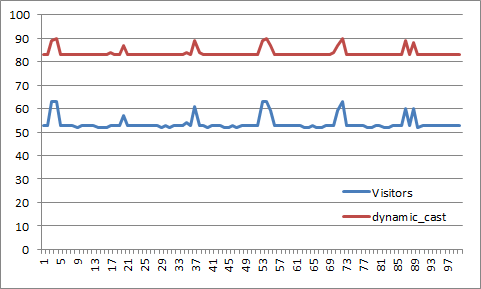
\includegraphics[width=0.47\textwidth]{DCast-vs-Visitors3.png}
  \caption{Time to uncover i\textsuperscript{th} case. X-axis - case i; Y-axis - cycles per iteration}
  \label{fig:DCastVis3}
\end{figure}

The most important benefit of this optimization, however, is the constant time 
on average used to dispatch each of the case clauses, regardless of their 
position in the type switch. The net effect of this optimization can be seen in Figure~\ref{fig:DCastVis3}. 
We can see that the time does not increase with the position of the case we are 
handling. The spikes represent activities on computer during measurement and are 
present in both measurements. 
The constant time on average comes from the average complexity 
of accessing an element in an \code{unordered_map}, while its worst complexity can 
be proportional to the size of the map. We show in the next section, however, 
that most of the time we will be bypassing traditional access to elements of the 
map, because, as-is, the type switch is still about 50\% slower than the visitor 
design pattern.

\noindent
Class \code{std::unordered_map} provides amortized constant time access on 
average and linear in the number of elements in the worst case. We show in the 
next section that most of the time we will be bypassing traditional access to 
its elements. We need this extra optimization because, as-is, the type switch is 
still about 50\% slower than the visitor design pattern.
\footnote{We are using 
speedups throughout the paper when comparing performance, so ``X is 42\% faster 
than Y'' or equally ``Y is 42\% slower than X'' means that Y's execution time is 
1.42 times X's execution time.}

Note that we can apply the reasoning of \textsection\ref{sec:memdev} and change 
the first-fit semantics of the resulting match statement into a best-fit 
semantics simply by changing the underlying cascading-if structure with decision 
tree. A compiler implementation of a type switch based on Vtable Pointer 
Memoization will certainly take advantage of this optimization to cut down the 
cost of the first run on a given vtbl-pointer, when the actual memoization happens.

Looking back at the example from \textsection\ref{sec:intro} and allowing for a few 
unimportant omissions, the first code snippet corresponds to what the macro 
\code{Match(x)} is expanded to when given a subject expression \code{x}. In order to 
see what \code{Case(Ti)} is expanded to, the second snippet has to be split on 
the line containing \code{si;} (excluding \code{si;} itself, which comes from 
source) and the second part (i.e. \} here) moved in front of the first one. The 
macro thus closes the scope of the previous case clause before starting the new 
one. \code{Case}'s expansion only relies on names introduced by \code{Match(x)}, 
its argument \code{Ti}, and a constant $i$, which can be generated from the
\code{__LINE__} macro, or, better yet, the \code{__COUNTER__} macro when 
supported by the compiler. The \code{EndMatch} macro simply closes the scopes 
(i.e. \}\} here). We refer the reader to the library source code for 
further details.

\subsubsection{Structure of Virtual Table Pointers}
\label{sec:sovtp}

Virtual table pointers are not entirely random addresses in memory and have 
certain structure when we look at groups of those that are associated with 
classes related by inheritance. Let us first look at some vtbl pointers that 
were present in some of our tests. The 32-bit pointers are shown in binary form 
(lower bits on the right) and are sorted in ascending order:

\begin{verbatim}
00000001001111100000011001001000
00000001001111100000011001011100
00000001001111100000011001110000
 ...
00000001001111100000011111011000
00000001001111100000011111101100
\end{verbatim}

Virtual table pointers are not constant values and are not even guaranteed to be 
the same between different runs of the same application. Techniques like 
\emph{address space layout randomization} or simple \emph{rebasing} of the entire 
module are likely to change these values. The relative distance between them is 
likely to remain the same though as long as they come from the same module.

Comparing all the vtbl pointers that are coming through a given match statement 
we can trace ar run time the set of bits in which they do and do not differ. 
For the above example it may look as \texttt{00000001001111100000X11XXXXXXX00} 
where positions marked with X represent bits that are different in some vtbl 
pointers.

When a DLL is loaded it may have its own copy of vtables for classes also used 
in other modules as well as vtables for classes it introduces. Comparing 
similarly all vtbl pointers coming only from this DLL we can get a different 
pattern \\ \texttt{01110011100000010111XXXXXXXXX000} and when compared over all 
the loaded modules the pattern will likely becomes something like 
\texttt{0XXX00X1X0XXXXXX0XXXXXXXXXXXXX00}.

The common bits on the right come from the virtual table size and alignment 
requirements, and, depending on compiler, configuration, and class hierarchy could 
easily vary from 2 to 6 bits. Because the vtbl-pointer under the C++ ABI points into 
an array of function pointers, the alignment requirement of 4 bytes for those 
pointers on a 32-bit architecture is what makes at least the last 2 bits to be 0. 
For our purpose the exact number of bits on the right is not important as we 
evaluate this number at run time based on vtbl-pointers seen so far. Here we only 
would like to point out that there would be some number of common bits on the 
right.

Another observation we made during our experiments with the vtbl-pointers of various 
existing applications was that the values of the pointers where changing more 
frequently in the lower bits than in the higher ones. We believe that this was 
happening because programmers tend to group multiple derived classes in the same 
translation unit so the compiler was emitting virtual tables for them close to 
each other as well. 

Note that derived classes that do not introduce their own virtual functions 
(even if they override some existing ones) are likely to have virtual tables of 
the same size as their base class. Even when they do add new virtual functions, 
the size of their virtual tables can only increase relative to their base 
classes. This is why the difference between many consecutive vtbl-pointers that 
came through a given match statement was usually constant or very slightly 
different.

The changes in higher bits were typically due to separate compilation and 
especially due to dynamically loaded modules. When a DLL is loaded, it may have 
its own copies of vtables for classes that are also used in other modules, in addition to 
vtables for classes it introduces. Comparing all vtbl-pointers coming only from 
that DLL we can get a different pattern \texttt{01110011100000010111XXXXXXXXX000} 
and when compared over all the loaded modules the pattern will likely become 
something like \texttt{0XXX00X1X0XXXXXX0XXXXXXXXXXXXX00}. Overall they were not 
changing the general tendency we saw: smaller bits were changing more frequently 
than larger ones, with the exception of the lowest common bits, of course.

These observations made virtual table pointers of classes related by inheritance 
ideally suitable for indexing -- the values obtained by throwing away the common 
bits on the right were compactly distributed in small disjoint ranges. We use 
those values to address a cache built on top of the hash table in order to 
eliminate a hash table lookup in most of the cases.  The important 
guarantee about the validity of the cached hash table references comes from the 
C++0x standard, which states that ``insert and emplace members shall not affect 
the validity of references to container elements''~\cite[\textsection 
23.2.5(13)]{C++0x}. 

Depending on the number of actual collisions that happen in the cache, our 
vtable pointer memoization technique can come close to, and even outperform, the 
visitor design pattern. The numbers are, of course, averaged over many runs as 
the first run on every vtbl-pointer will take an amount of time as shown in 
Figure\ref{fig:DCastVis1}. We did however test our technique on real code and 
can confirm that it does perform well in the real-world use cases.

The information about jump targets and necessary offsets is just an example of 
information we might want to be able to associate with, and access via, virtual 
table pointers. Our implementation of \code{memoized_cast} from 
\textsection\ref{sec:memcast} effectively reuses this general data structure with 
a different type of element values. We thus created a generic reusable class 
\code{vtblmap<T>} that maps vtbl-pointers to elements of type T. We will refer 
to the combined cache and hash-table data structure, extended with the logic for 
minimizing conflicts presented below, as a \emph{vtblmap} data structure.

\subsection{Minimization of Conflicts}
\label{sec:moc}

Virtual table pointers are not constant values and are not even guaranteed to be 
the same between different runs of the application, because techniques like 
\emph{address space layout randomization} or \emph{rebasing} of the module are 
likely to change them. The relative distance between them will remain the same 
as long as they come from the same module.

Knowing that vtbl-pointers point into an array of function pointers, we should 
expect them to be aligned accordingly and thus have a few lowest bits as zero. 
Moreover, since many derived classes do not introduce new virtual functions, 
the size of their virtual tables remains the same. When allocated sequentially 
in memory, we can expect a certain number of lowest bits in the vtbl-pointers 
pointing to them to be the same.
These assumptions, supported by actual observations, made virtual table 
pointers of classes related by inheritance ideally suitable for hashing: the 
values obtained by throwing away the common bits on the right were compactly 
distributed in small disjoint ranges (\textsection\ref{sec:hierarchies}). We use 
them to address a cache built on top of the hash table in order to eliminate a 
hash table lookup in most of the cases.

Let $\Xi$ be the domain of integral representations of pointers. Given a cache 
with $2^k$ entries, we use a family of hash functions $H_{kl} : \Xi \rightarrow [0..2^k-1]$ 
defined as $H_{kl}(v)=v/2^l \mod 2^k$ to index the cache, where $l \in [0..32]$ 
(assuming 32 bit addresses) is a parameter modeling the number of common bits on 
the right. Division and modulo are implemented with bit operations since the
denominator in each case is a power of 2, which in turn explains the choice of 
the cache size.

Given a hash function $H_{kl}$, pointers $v'$ and $v''$ are said to be in 
\emph{conflict} when $H_{kl}(v')=H_{kl}(v'')$. For a given set of pointers 
$V \in 2^{\Xi}$, we can always find such $k$ and $l$ that $H_{kl}$ will render no  
conflicts between its elements, but the required cache size $2^k$ can be too 
large to justify the use of memory. The value $K$ such that $2^{K-1} < |V| \leq 2^K$ 
is the smallest value of $k$ under which absence of conflicts is still possible. 
We thus allow $k$ to vary only in the range $[K,K+1]$ to ensure that the cache size 
is never more than 4 times bigger than the minimum required cache size.

Given a set $V = \{v_1, ... , v_n\}$, we would like to find a pair of parameters 
$(k,l)$ such that $H_{kl}$ will render the least number of conflicts on the 
elements of $V$. Since for a fixed set $V$, parameters $k$ and $l$ vary in a 
finite range, we can always find the optimal $(k,l)$ by trying all the
combinations. Let $H_{kl}^V : V \rightarrow [0..2^k-1]$ be the hash function 
corresponding to such optimal $(k,l)$ for the set $V$. 

In our setting, the set $V$ represents the set of vtbl-pointers coming through a 
particular type switch. While the exact values of these pointers are not known 
until run-time, their offsets from the module's base address are. This is generally 
sufficient to estimate optimal $k$ and $l$ in a compiler setting. In the library 
setting, we recompute them after a given number of actual collisions in cache.

When $H_{kl}^V$ is injective (renders 0 conflicts on $V$), the frequency of any 
given vtbl-pointer $v_i$ coming through the type switch does not affect the 
overall performance of the switch. However when $H_{kl}^V$ is not injective, we 
would prefer the conflict to happen on less frequent vtbl-pointers.
Given a probability $p(v_i)$ of each vtbl-pointer $v_i \in V$ we can compute the 
probability of conflict rendered by a given $H_{kl}$:

\begin{eqnarray*}
p_{kl}(V)=\sum\limits_{j=0}^{2^k-1}\of{\sum\limits_{v_{i} \in V^j_{kl}}p(v_i)}\of{1-\frac{\sum\limits_{v_i \in V^j_{kl}}p(v_i)^2}{\of{\sum\limits_{v_{i} \in V^j_{kl}}p(v_i)}^2}}
\end{eqnarray*}

\noindent 
where $V^j_{kl}=\{v \in V | H_{kl}(v)=j\}$. In this case, the optimal hash 
function $H_{kl}^V$ can similarly be defined as $H_{kl}$ that minimizes the 
above probability of conflict on $V$.

The probabilities $p(v_i)$ can be estimated in a compiler setting through profiling, 
while in a library setting we let the user enable tracing of frequencies of 
each vtbl-pointer. This introduces an overhead of an increment into the critical 
path of execution, and according to our tests degrades the performance by 1-2\%. 
This should not be a problem as long as the overall performance gains from a
smaller probability of conflicts happening at run time. Unfortunately, in our 
tests the significant drop in the number of actual collisions was not reflected 
in a noticeable decrease in execution time, which is why we do not enable 
frequency tracing by default. As we will see in \textsection\ref{sec:hierarchies}, 
this was because the hash function $H_{kl}^V$ renders no conflicts on 
vtbl-pointers in most cases and the few collisions we were getting before 
inferring the optimal $k$ and $l$ even in non-frequency-based caching where 
incomparably smaller than the number of successful cache hits.

Assuming uniform distribution of $v_i$ in $V$ and substituting the probability 
$p(v_i)=\frac{1}{n}$, where $n=|V|$, into the above formula we get:

\begin{eqnarray*}
p_{kl}(V)=\sum\limits_{j=0}^{2^k-1}[|V^j_{kl}| \neq 0]\frac{|V^j_{kl}|-1}{n}
\end{eqnarray*}

\noindent
We use the Iverson bracket $[\pi]$ here to refer to the outcome of a predicate $\pi$ as numbers $0$ or $1$.
The value $|V^j_{kl}|$ represents the number of vtbl-pointers $v_i \in V$ that are mapped to the same location $j$ in cache with $H_{kl}^V$. Only 
one such vtbl-pointer will actually be present in that cache location at any given 
time, which is why the value $|V^j_{kl}|-1$ represents the number of ``extra'' 
pointers mapped into the entry $j$ on which a collision will happen. The overall 
probability of conflict thus only depends on the total number of these ``extra'' 
or conflicting vtbl-pointers. The $H_{kl}^V$ obtained by minimization of 
probability of conflict under uniform distribution of $v_i$ in $V$ is thus the 
same as the original $H_{kl}^V$ that was minimizing the number of conflicts. An 
important observation here is that since the exact location of these ``extra'' 
vtbl-pointers is not important and only the total number $m$ is, the probability 
of conflict under uniform distribution of $v_i$ in $V$ is always going to be of 
the discrete form $\frac{m}{n}$, where $0 \le m < n$.

%Depending on the number of actual collisions that happen in the cache, our 
%vtable pointer memoization technique can come close to, and even outperform, the 
%visitor design pattern. The numbers are, of course, averaged over many runs as 
%the first run on every vtbl-pointer will take an amount of time as shown in 
%Figure\ref{fig:DCastVis1}. We did however test our technique on real code and 
%can confirm that it does perform well in the real-world use cases.

%The information about jump targets and necessary offsets is just an example of 
%information we might want to be able to associate with, and access via, virtual 
%table pointers. Our implementation of \code{memoized_cast}~\cite[\textsection 9]{TR}, for example, 
%effectively reuses this general data structure with a different type of element 
%values. We thus created a generic reusable class \code{vtblmap<T>} that maps 
%vtbl-pointers to elements of type T. We will refer to the combined cache and 
%hash-table data structure, extended with the logic for minimizing conflicts 
%presented below, as a \emph{vtblmap} data structure.

%\subsubsection{Minimization of Conflicts}
%\label{sec:moc}

The small number of cycles that the visitor design pattern needs to uncover a 
type does not let us put too sophisticated cache indexing mechanisms into the 
critical path of execution. This is why we limit our indexing function to shifts 
and masking operations as well as choose the size of the cache to be a power of 2.

Throughout this section by \emph{collision} we will call a run-time condition in 
which the cache entry of an incoming vtbl pointer is occupied by another vtbl-pointer.
Collision requires vtblmap to fetch the data associated with the new 
vtbl-pointer from a slower hash-table and, under certain conditions, reconfigure 
cache for better performance. By \emph{conflict} we will call a different 
run-time condition under which given cache configuration maps two or more vtbl 
pointers to the same cache location. Presence of conflict does not necessarily 
imply presence of collisions, but collisions can only happen when there is a 
conflict. In the rest of this section we devise a mechanism that tries to 
minimize the amount of conflicts in a hope that it will also decrease the amount 
of actual collisions.

Given $n$ vtbl-pointers we can always find a cache size that will render no 
conflicts between them. The necessary size of such a cache, however, can be too 
big to justify the use of memory. This is why, in our current implementation, we 
always consider only 2 different cache sizes: $2^k$ and $2^{k+1}$ where 
$2^{k-1} < n \leq 2^k$. This guarantees that the cache size is never more than 4 
times bigger than the minimum required cache size.

During our experiments, we noticed that often the change in the smallest 
different bit happens only in a few vtbl-pointers, which was effectively 
cutting the available cache space in half. To overcome this problem, we let the 
number of bits by which we shift the vtbl-pointer vary further and compute it in 
a way that minimizes the number of conflicts.

To avoid doing any computations in the critical path, \code{vtblmap} only 
recomputes the optimal shift and the size of the cache when an actual collision 
happens. In order to avoid constant recomputations when conflicts are unavoidable, 
we add an additional restriction of only reconfiguring the optimal parameters if 
the number of vtbl-pointers in the \code{vtblmap} has increased since the last 
recomputation. Since the number of vtbl-pointers is of the order $O(|A|)$, where 
$A$ is the static type of all vtbl-pointers coming through a \code{vtblmap}, the 
restriction assures that reconfigurations will not happen infinitely often.

To minimize the number of recomputations even further, our library communicates 
to the \code{vtblmap}, through its constructor, the number of case clauses in 
the underlying match statement. We use this number as an estimate of the expected 
size of the \code{vtblmap} and pre-allocate the cache according to this estimated 
number. The cache is still allowed to grow based on the actual number of 
vtbl-pointers that comes through a \code{vtblmap}, but it never shrinks from the
initial value. This improvement significantly minimizes the number of collisions 
at early stages, as well as the number of possibilities we have to consider 
during reconfiguration.

The above logic of \code{vtblmap} always chooses the configuration that renders 
no conflicts, when such a configuration is possible during recomputation of 
optimal parameters. When this is not possible, it is natural to prefer collisions 
to happen on less-frequent vtbl-pointers.

We studied the frequency of vtbl-pointers that come through various match statements
of a C++ pretty-printer that we implemented on top of the Pivot 
framework~\cite{Pivot09} using our pattern-matching library. We ran the 
pretty-printer on a set of C++ standard library headers and then ranked all the  
classes from the most-frequent to the least-frequent ones, on average. The 
resulting probability distribution is shown with a thicker line in 
Figure\ref{fig:PowerLaw}.

\begin{figure}[htbp]
  \centering
    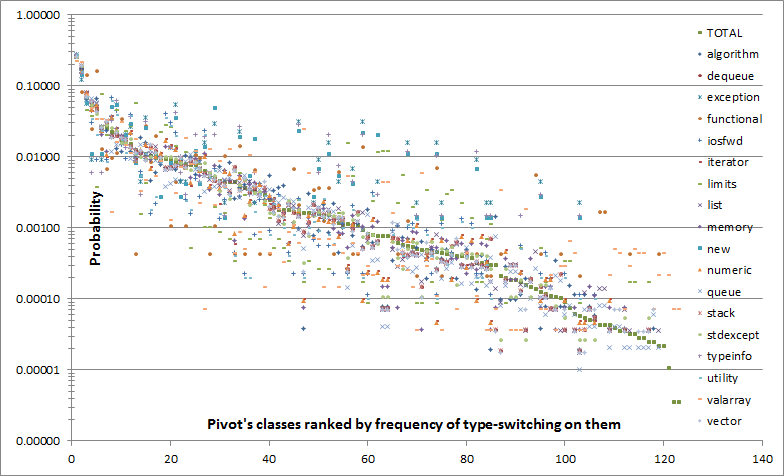
\includegraphics[width=0.47\textwidth]{std-lib-power-law-distributions.png}
  \caption{Probability distribution of various nodes in Pivot framework}
  \label{fig:PowerLaw}
\end{figure}

Note that Y-Axis is using logarithmic scale, suggesting that the resulting 
probability has power-law distribution. This is likely to be a specifics of our 
application, nevertheless, the above picture demonstrates that frequency of certain 
classes can be larger than the overall frequency of all the other classes. In 
our case, the two most frequent classes were representing the use of a variable in 
a program, and their combined frequency was larger than the frequency of all the 
other nodes. Naturally, we would like to avoid conflicts on such classes in the 
cache, when possible.

Let us assume that a given \code{vtblmap} contains a set of vtbl pointers 
$V = \{v_1, ... , v_n\}$ with known probabilities $p_i$ of occuring. For a cache 
of size $2^k$ and a shift by $l$ bits we get a cache-indexing function 
$f_{lk} : V \rightarrow [0..2^k-1]$ defined as $f_{lk}(v_i) = (v_i \gg l) \& (2^k-1)$.
To calculate the probability of conflict for a given $l$ and $k$ parameters, let 
us consider $j^{th}$ cache cell and a subset $V^j_{lk}=\{v \in V | f_{lk}(v)=j\}$. 
When the size of this subset $m=|V^j_{lk}|$ is greater than 1, we have a 
potential conflict as subsequent request for a vtbl pointer $v''$ might be 
different from the vtbl pointer $v'$ currenly stored in the cell $j$. Within the 
cell only the probability of not having a conflict is the probability of both 
values $v''$ and $v'$ be the same:
\begin{eqnarray*}
P(v''=v')=\sum\limits_{v_i \in V^j_{lk}}P(v''=v_i)P(v'=v_i)=\sum\limits_{v_i \in V^j_{lk}}P^2(v_i|V^j_{lk})=\\
=\sum\limits_{v_i \in V^j_{lk}}\frac{P^2(v_i)}{P^2(V^j_{lk})}=
\sum\limits_{v_i \in V^j_{lk}}\frac{p_i^2}{(\sum\limits_{v_{i'} \in V^j_{lk}}p_{i'})^2}=
\frac{\sum\limits_{v_i \in V^j_{lk}}p_i^2}{(\sum\limits_{v_{i} \in V^j_{lk}}p_{i})^2}
\end{eqnarray*}

The probability of having a conflict among the vtbl pointers of a given cell is 
thus one minus the above value:

\begin{eqnarray*}
P(v''\neq v')=1-\frac{\sum\limits_{v_i \in V^j_{lk}}p_i^2}{(\sum\limits_{v_{i} \in V^j_{lk}}p_{i})^2}
\end{eqnarray*}

To obtain probability of conflict given any vtbl pointer and not just the one 
from a given cell we need to sum up the above probabilities of conflict within a 
cell multiplied by the probability of vtbl pointer fall into that cell:

\begin{eqnarray*}
P_{lk}^{conflict}=\sum\limits_{j=0}^{2^k-1}P(V^j_{lk})(1-\frac{\sum\limits_{v_i \in V^j_{lk}}p_i^2}{(\sum\limits_{v_{i} \in V^j_{lk}}p_{i})^2})=\\
=\sum\limits_{j=0}^{2^k-1}(\sum\limits_{v_{i} \in V^j_{lk}}p_{i})(1-\frac{\sum\limits_{v_i \in V^j_{lk}}p_i^2}{(\sum\limits_{v_{i} \in V^j_{lk}}p_{i})^2})
\end{eqnarray*}

Our reconfiguration algorithm then iterates over possible values of $l$ and $k$ 
and chooses those that minimize the overal probability of conflict $P_{lk}^{conflict}$.
The only data still missing are the actual probabilities $p_i$ used by the above 
formula. They can be approximated in many different ways.

Besides probability distribution on all the tests, Figure~\ref{fig:PowerLaw} 
shows probabilities of a given node on each of the tests. The X-Axis in this 
case represents the ordering of all the nodes according to their overall rank 
of all the tests combined. As can be seen from the picture, the shape of each 
specific test's distribution still mimics the overal probability distribution. 
With this in mind we can simply let the user assign probabilities to each of the 
classes in the hierarchy and use these values during reconfiguration. The 
practical problem we came accross with this solution was that we wanted these 
probabilities be inheritable as Pivot separates interface and implementation 
classes and we prefered the user to define them on interfaces rather than on 
implementation classes. The easiest way to do so wast to write a dedicated 
function that would return the probabilities using a match statement. 
Unfortunately such a function will introduce a lot of overhead as it will 
ideally only be used very few times (since we try to minimize the amount of 
reconfiguration) and thus not be using memoized jumps but rather slow 
cascading-if.

A simpler and likely more precise way of estimating $p_i$ would be to count 
frequencies of each vtbl pointers directly inside the \code{vtblmap}. This 
introduces an overhead of an increment into the critical path of execution, but 
according to our tests was only degrading the overal performance by 1-2\%.
Instead, it was compensating with a smaller amount of conflicts and thus a 
potential gain of performance. We leave the choice of whether the library should 
count frequencies of each vtbl pointer to the user of the library as the 
concrete choice may be to advantage on some class hierarchies and to 
disadvantage on others.

Figure~\ref{fig:Collisions} compares the amount of collisions when frequency 
information is and is not used. The data was gathered from 312 tests on multiple 
match statements present in Pivot's C++ pretty printer when it was ran over 
standard library headers. In 122 of these test both schemes had 0 conflicts and 
these tests are thus not shown on the graph. The remaining tests where ranked by 
the amount of conflicts in the scheme that does not utilize frequency information.

\begin{figure}[htbp]
  \centering
    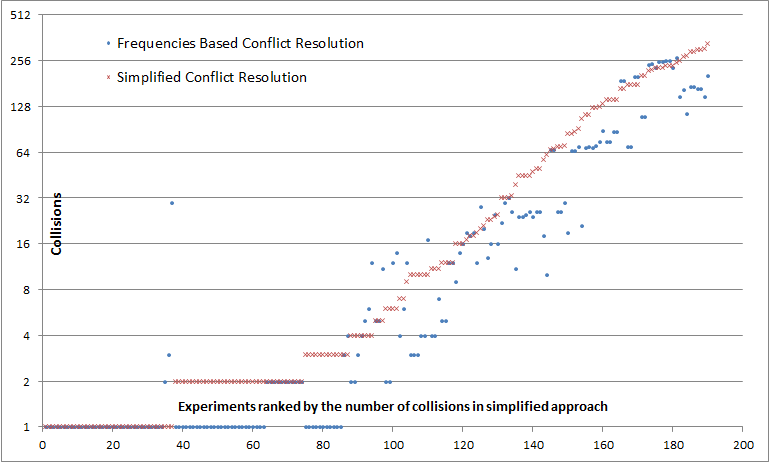
\includegraphics[width=0.47\textwidth]{CollisionsWithAndWithoutFrequencies.png}
  \caption{Decrease in number of collisions when probabilities of nodes are taken into account}
  \label{fig:Collisions}
\end{figure}

As can be seen from the graph, both schemes render quite low amount of 
collisions given that there was about 57000 calls in the rightmost test having 
the largest amount of conflicts. Taking into account that the Y-axis has 
logarithmic scale, the use of frequency information in many cases decreased the 
amount of conflicts by a factor of 2. The handfull of cases where the use of 
frequency increased the number of conflicts can be explained by the fact that 
the optimal values are not recomputed after each conflict, but after several 
conflicts and only if the amount of vtbl pointers in the vtblmap increased. These 
extra conditions sacrify optimality of parameters at any given time for the amount 
of times they are recomputed. By varying the number of conflicts we are willing 
to tolerate before reconfiguration we can decrease the number of conflicts by 
increasing the amount of recomputations and vise versa. From our experience, 
however, we saw that the drop in the number of conflicts was not translating 
into a proportional drop in execution time, while the amount of reconfigurations 
was proportional to the increase in execution time. This is why we choose to 
tolerate a relatively large amount of conflicts before recomputation just to 
keep the amount of recomputations low.
